%! TEX root = ../main.tex
% ==============================================================
% IMMUTABLE — generated automatically, do not edit this block
%
% — Provenance ───────────────────────────────────────────────────
%   script            : analysis_scratch/hg_per40_window_fitness.py
%   computed_in       : analysis_scratch/hg_per40_window_fitness.py (proposed H&G formula: t_start = r/c_g(f,h) + 15/f, length 10T, start snapped to nearest upcrossing within ±T)
%   plot_type         : hg_per40_window_fitness
%   data_class        : DFS
%   generated_at      : 2026-05-03T16:49:12
%   findings_doc      : 
%
% — Thesis context ──────────────────────────────────────────────
%   chapter           : 04
%   caption_label     : fig:ch04_hg_per40_window_fitness_f13
%   caption_short     : 
%
% — Filters ────────────────────────────────────────────────────
%   panel             : full
%   wind              : no, full
%   amplitude [V]     : 0.2
%   frequency [Hz]    : 1.3
%   probes            : 
%   run_category      : 
%   quality_flag      : ok
%   mooring           : 
%
% — Data provenance ────────────────────────────────────────────
%   n_runs            : 5
%   in_probes_used    : 9373/170+9373/340
%   out_probes_used   : 12400/250
%   probe_configs     : march2026_better_rearranging
%   non_final_config_n: 
%   datasets        :
%     PROCESSED-20260326-ProbePos4_31_FPV_2-tett6roof-under9Mooring-height100-lowrange
%     PROCESSED-20260327-ProbePos4_31_FPV_2-tett6roof-under9Mooring30-height100-lowrange
%   run_paths       :
%     wavedata/20260326-ProbePos4_31_FPV_2-tett6roof-under9Mooring-height100-lowrange/fullpanel-fullwind-amp0200-freq1300-per240-depth580-mstop30-run1.csv
%     wavedata/20260327-ProbePos4_31_FPV_2-tett6roof-under9Mooring30-height100-lowrange/fullpanel-nowind-amp0200-freq1300-per240-depth580-mstop30-run1.csv
%     wavedata/20260327-ProbePos4_31_FPV_2-tett6roof-under9Mooring30-height100-lowrange/fullpanel-fullwind-amp0200-freq1300-per240-depth580-mstop30-run1.csv
%     wavedata/20260327-ProbePos4_31_FPV_2-tett6roof-under9Mooring30-height100-lowrange/fullpanel-fullwind-amp0200-freq1300-per40-depth580-mstop30-run1.csv
%     wavedata/20260327-ProbePos4_31_FPV_2-tett6roof-under9Mooring30-height100-lowrange/fullpanel-nowind-amp0200-freq1300-per40-depth580-mstop30-run1.csv
%
% — Method / numerical parameters ─────────────────────────────
%   grouper           : one representative run per (run_type × wind) cell
%   collapse_panels   : False
%   fft_window_hz     : 
%   extra_params      : f_paddle = 1.3 Hz; N_offset = 15 periods; window length = 10 T; r_IN = 9.373 m, r_OUT = 12.4 m; depth = 0.58 m
%
% — Summary stats cited in caption ────────────────────────────
%   stat:theoretical_IN_window_s : [27.07, 34.76]
%   stat:theoretical_OUT_window_s : [32.08, 39.77]
%   stat:n_per40_in_cohort : 2
%   stat:n_per240_in_cohort : 3
%
% — Subfigures available ───────────────────────────────────────
%     FIGURES/ch04_hg_per40_window_fitness_f13.pdf
% ── end immutable block ─────────────────────────────────────────
\begin{figure}[htbp]
  \centering
  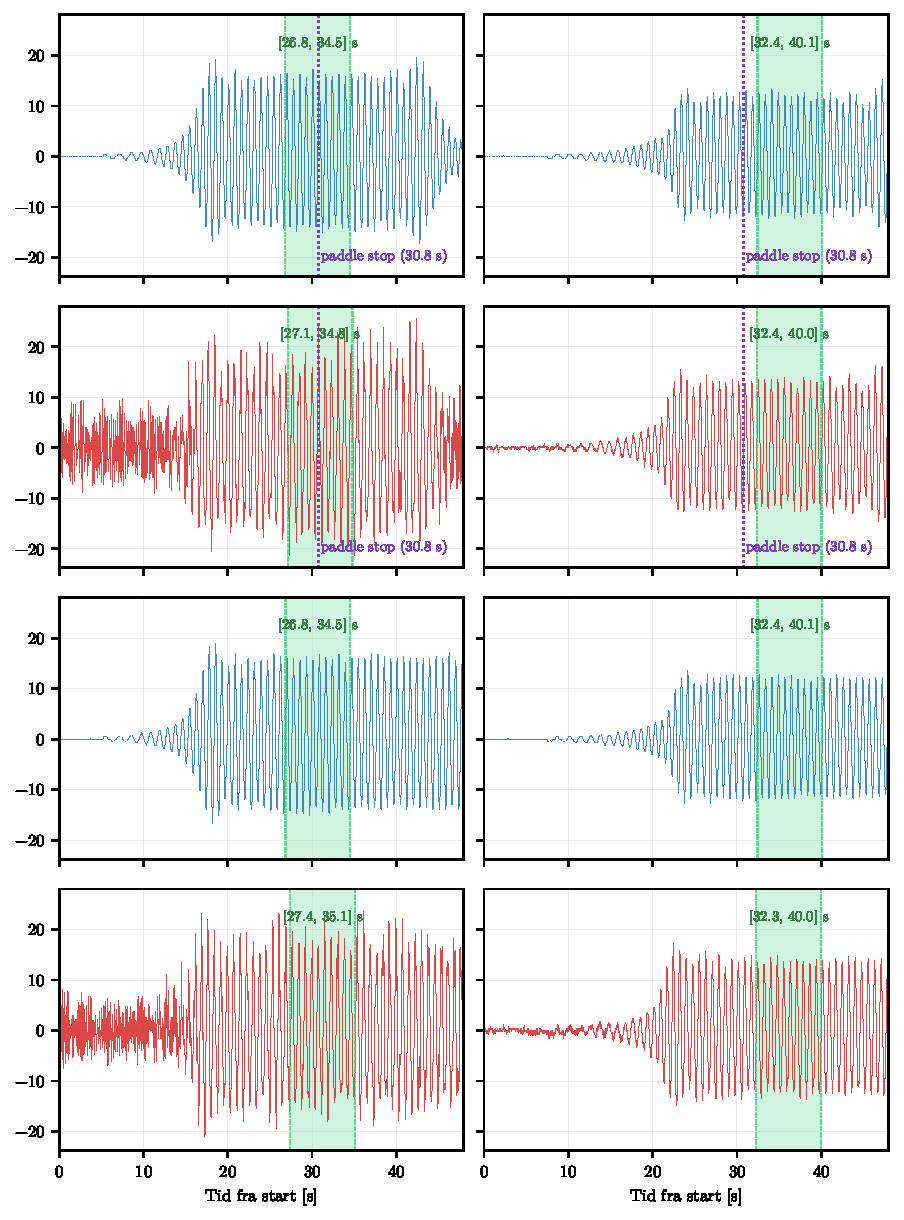
\includegraphics[width=\linewidth]{FIGURES/ch04_hg_per40_window_fitness_f13.pdf}
  \caption{
    % TODO: write caption
  }
  \label{fig:ch04_hg_per40_window_fitness_f13}
\end{figure}
